\documentclass[cover.tex]{subfiles}

 \begin{document} \begin{refsection}

\taburulecolor{black}

%%%%%%%%%%%%HEADING TITLE
\hfill\vspace{0.2cm}\begin{center}{\large \bfseries EXPERIMENT \par\Huge
 \import{\labname/}{title}
 \\[5pt] \par}\vspace{0.2cm}\end{center}\par\noindent
 %%%%%%%%%%%%HEADING
 
 
\section*{Goal}
 \import{\labname/}{goal}
\section*{Materials}
 \import{\labname/}{materials}
\section*{Background}
%\import{\labname/}{video}

\import{\labname/}{background}


%\import{\labname/}{examplebox}
%%%%%BIBLIOGRAPHY
\printbibliography[heading=subbibliography]
%%%%%BIBLIOGRAPHY
%\section*{Lab Information}
% \begin{itemize}[label={$\blacksquare$}]
 %  \import{\labname/}{labinfo}
% \end{itemize}
\section*{Procedure}
\import{\labname/}{procedure} 


%\clearpage\mbox{}\clearpage



%%%%%%%%%%%%HEADING
\newgeometry{right=5cm}\thispagestyle{sidebar}\sidebar{   \vspace{1em}\vspace{1cm} \vfill \par\vspace*{1em}}\restoregeometry\clearpage \begin{multicols}{2}\begin{tcolorbox}[enhanced jigsaw,breakable,size=title,colback=mybrown!05,colframe=black,fonttitle=\bfseries,title=STUDENT INFO,pad at break=1mm, break at=15cm/0pt ]\vspace{0.2cm}\noindent Name:  \begin{Form}\TextField[name=NAME, width=4cm,height=0.5cm,multiline=false, borderstyle=U, bordercolor={black}]{} \end{Form}   \hspace{0.2cm}Date:  \begin{Form}\TextField[name=DATE, width=1.5cm,height=0.5cm,multiline=false, borderstyle=U, bordercolor={black}]{}\end{Form} \\\end{tcolorbox}\end{multicols}\hfill\vspace{0.2cm}\begin{center}{\large \bfseries Pre-lab Questions \par\Huge
\import{\labname/}{title}
\\[5pt] \par}\vspace{0.2cm}\end{center}\par\noindent\uline{  \hfill \normalsize \hfill       }
%%%%%%%%%%%%HEADING

\import{\labname/}{prelab}

%%%%%%%%%%%%%HEADING
%\newgeometry{right=5cm}\thispagestyle{sidebar}\sidebar{ \vspace{1em} \vspace{1cm}\vfill\par\vspace*{1em}}\restoregeometry\clearpage\begin{sidewaystable}[ph!]\begin{multicols}{2}\begin{tcolorbox}[enhanced jigsaw,breakable,size=title,colback=mybrown!05,colframe=black,fonttitle=\bfseries,title=STUDENT INFO,pad at break=1mm, break at=15cm/0pt ]\vspace{0.2cm}\noindent Name:  \begin{Form}\TextField[name=NAME, width=4cm,height=0.5cm,multiline=false, borderstyle=U, bordercolor={black}]{} \end{Form}   \hspace{0.2cm}Date:  \begin{Form}\TextField[name=DATE, width=1.5cm,height=0.5cm,multiline=false, borderstyle=U, bordercolor={black}]{}\end{Form} \\\end{tcolorbox}\end{multicols}\hfill\vspace{-1cm}\begin{center}{\large \bfseries Results\\ EXPERIMENT \par\Huge
%\import{\labname/}{title}
%\\[5pt] \par}\vspace{0.2cm}\end{center}\par\noindent
%%%%%%%%%%%%%HEADING

%%%%%%%%%%%%HEADING
\newgeometry{right=5cm}
\thispagestyle{sidebar}
\sidebar{%
  \vspace{1em}
  \vspace{1cm}
  \vfill
  \par\vspace*{1em}
}
\restoregeometry
\clearpage 
 
\begin{sidewaystable}[ph!]  \vspace{1cm}
\begin{multicols}{2}
\begin{tcolorbox}[enhanced jigsaw,breakable,size=title,
colback=mybrown!05,colframe=black,fonttitle=\bfseries,
title=STUDENT INFO,pad at break=1mm, break at=5cm/0pt ]
\vspace{0.2cm}
\noindent Name:  \begin{Form}\TextField[rotation=90,name=NAME, width=4cm,height=0.5cm,multiline=false, borderstyle=U, bordercolor={black}]{} \end{Form}   \hspace{0.2cm}Date:  \begin{Form}\TextField[rotation=90, name=DATE, width=1.5cm,height=0.5cm,multiline=false, borderstyle=U, bordercolor={black}]{}\end{Form} \\
\end{tcolorbox}
\hfill
\vspace{1cm}
\begin{center}
{\large \bfseries  
Results\\ EXPERIMENT  
\par
\Huge
\import{\labname/}{title}
\\[5pt] \par}
\vspace{0.2cm}
\end{center}
\par
\noindent
\end{multicols}


\hspace{-2cm}\vspace{-1cm}

 \import{\labname/}{results}
\end{sidewaystable}


\newpage
\begin{sidewaystable}[ph!]  \vspace{1cm}
\import{\labname/}{results1}
\end{sidewaystable}

%\clearpage\mbox{}\clearpage
%\vspace{1cm}
%\begin{sidewaystable}[ph!]  \vspace{1cm}
%\import{\labname/}{results2}
%\end{sidewaystable}
%\clearpage\mbox{}\clearpage

\newpage
\clearpage\mbox{}\clearpage
\begin{center}
 \vspace{2cm}
 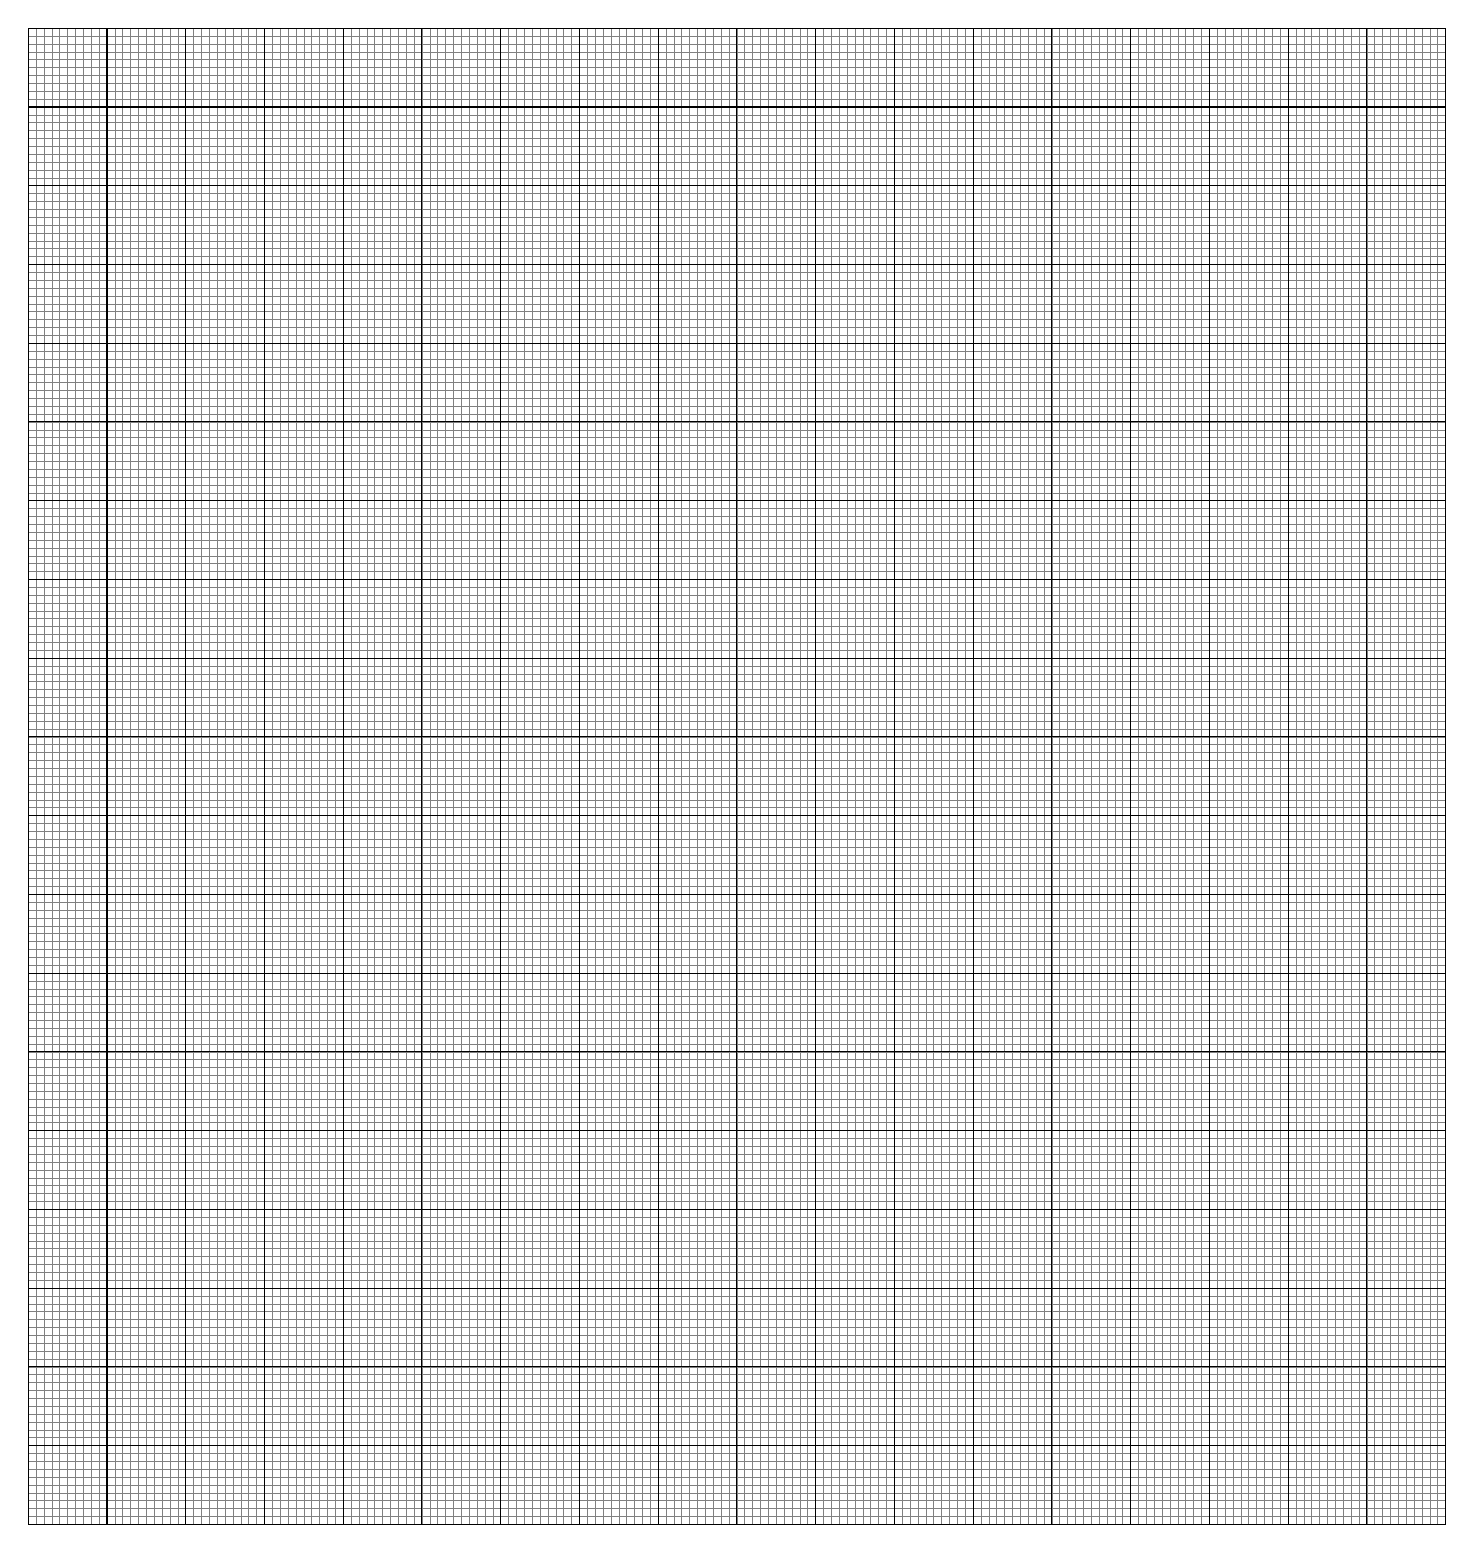
\begin{tikzpicture}
 \draw[step=1mm,help lines] (0,0) grid (180mm,190mm);
 \draw[step=10mm] (0,0) grid (180mm,190mm);
\end{tikzpicture}\\\captionof{figure}{$\overline{A}$ cps (Y axis) vs. N (X axis)}\end{center}


%%%%%%%%%%%%HEADING
\newgeometry{right=5cm}\thispagestyle{sidebar}\sidebar{\vspace{1em}\vspace{1cm}\vfill\par\vspace*{1em}}\restoregeometry\clearpage \begin{multicols}{2}\begin{tcolorbox}[enhanced jigsaw,breakable,size=title,colback=mybrown!05,colframe=black,fonttitle=\bfseries,title=STUDENT INFO,pad at break=1mm, break at=15cm/0pt ]\vspace{0.2cm}\noindent Name:  \begin{Form}\TextField[name=NAME, width=4cm,height=0.5cm,multiline=false, borderstyle=U, bordercolor={black}]{} \end{Form}   \hspace{0.2cm}Date:  \begin{Form}\TextField[name=DATE, width=1.5cm,height=0.5cm,multiline=false, borderstyle=U, bordercolor={black}]{}\end{Form} \\\end{tcolorbox}\end{multicols}\hfill\vspace{0.2cm}\begin{center}{\large \bfseries Post-lab Questions \par\Huge
 \import{\labname/}{title}
\\[5pt] \par}\vspace{0.2cm}\end{center}\par\noindent\uline{  \hfill \normalsize \hfill       }
%%%%%%%%%%%%HEADING
 \import{\labname/}{postlab}
\clearpage\mbox{}\clearpage

 \end{refsection}
\end{document}
